\section{Comparison Clustering} \label{sec:Comparison_Clustering}

\blindtext

\begin{figure}[!hbt]
    \centering
    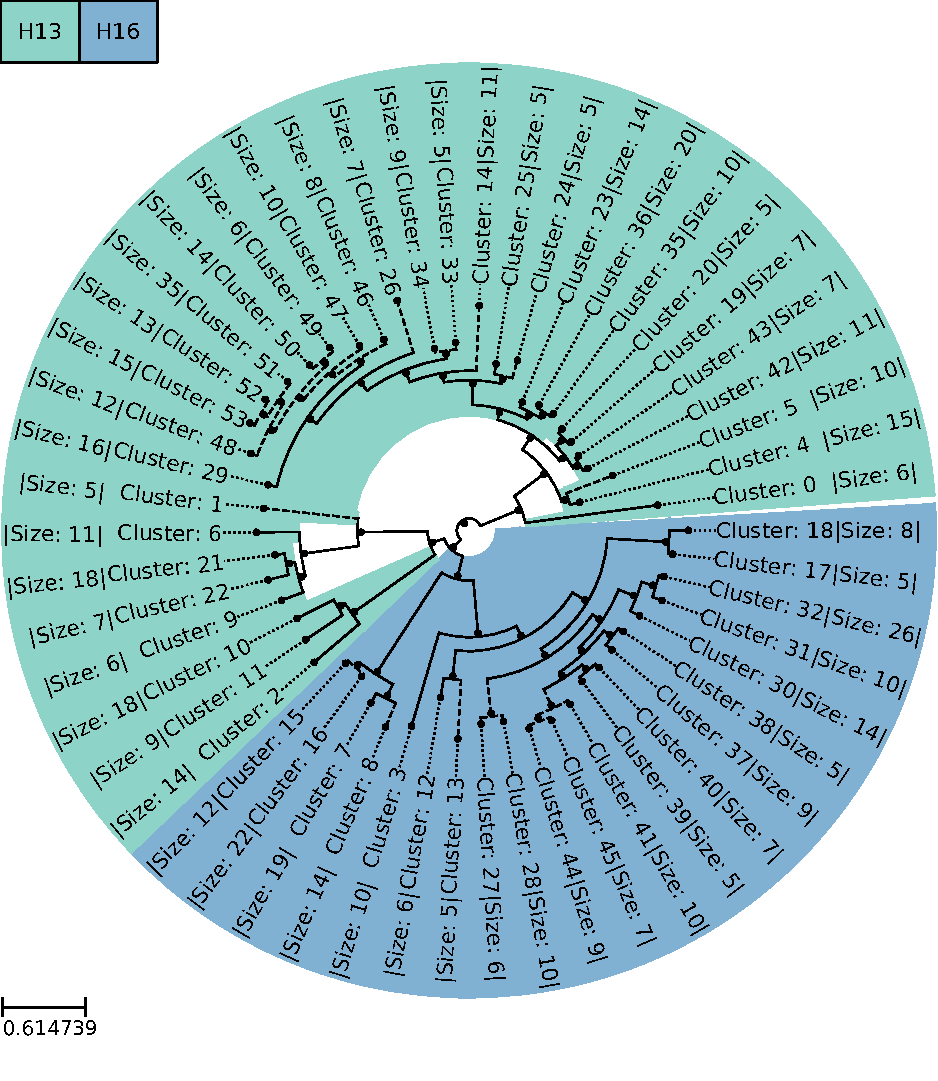
\includegraphics[width=\textwidth]{PCA/Clustertree_Segment_4_H_Simple.pdf}
    \caption[H13/H16 Simple Clustering Example (\Acrshort{PCA})]{\textbf{H13/H16 Simple Clustering Example (\Acrshort{PCA}).} .}
    \label{fig:Simple_Clustertree_PCA}
\end{figure}

\begin{figure}[!hbt]
    \centering
    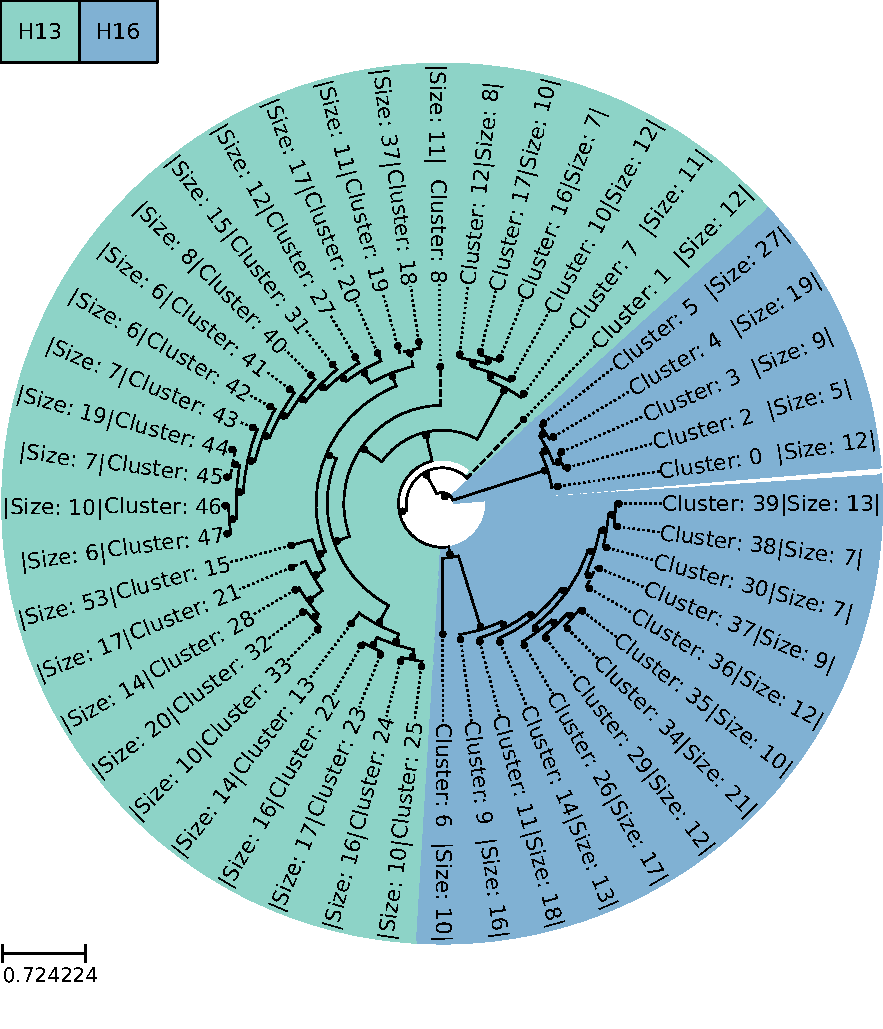
\includegraphics[width=\textwidth]{UMAP/Clustertree_Segment_4_H_Simple.pdf}
    \caption[H13/H16 Simple Clustering Example (\Acrshort{UMAP})]{\textbf{H13/H16 Simple Clustering Example (\Acrshort{UMAP}).} .}
    \label{fig:Simple_Clustertree_UMAP}
\end{figure}

\begin{figure}[!hbt]
    \centering
    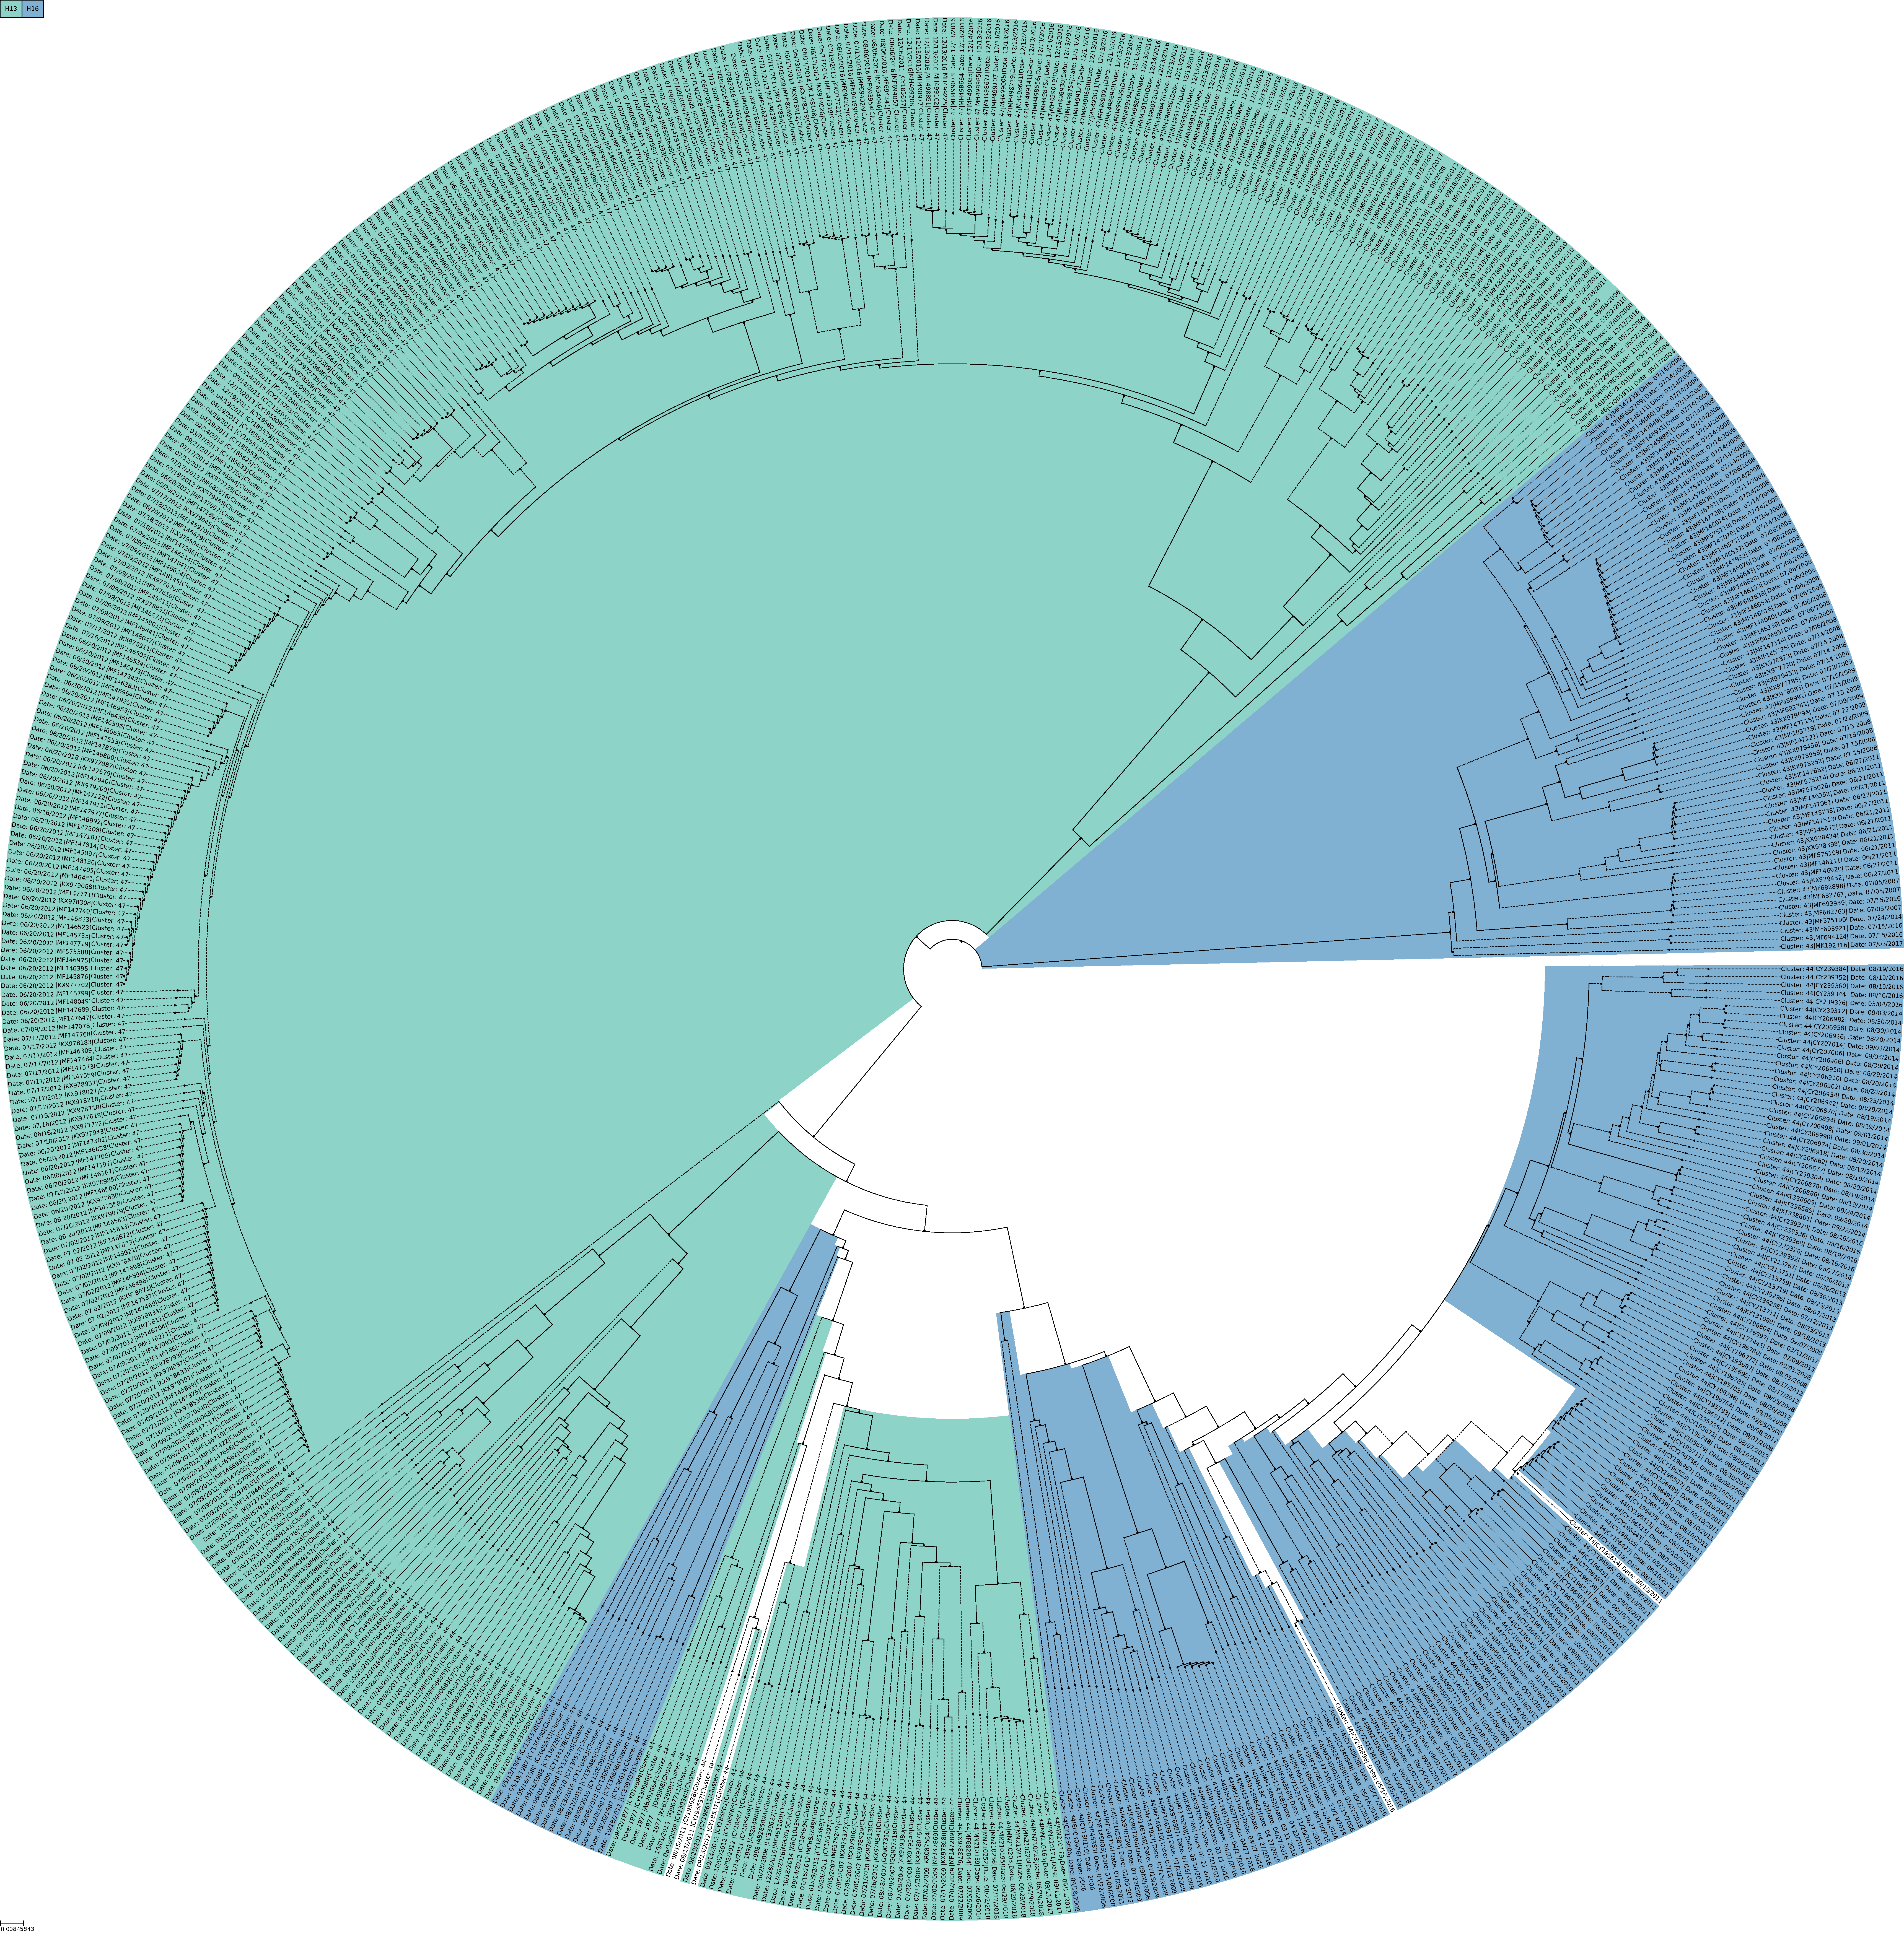
\includegraphics[width=\textwidth]{PCA/Clustertree_Segment_4_H_Focus.pdf}
    \caption[H13/H16 Simple Clustering Example with Guidetree]{\textbf{H13/H16 Simple Clustering Example with Guidetree.} .}
    \label{fig:Simple_Clustertree_MSA}
\end{figure}

\begin{figure}[!hbt]
    \centering
    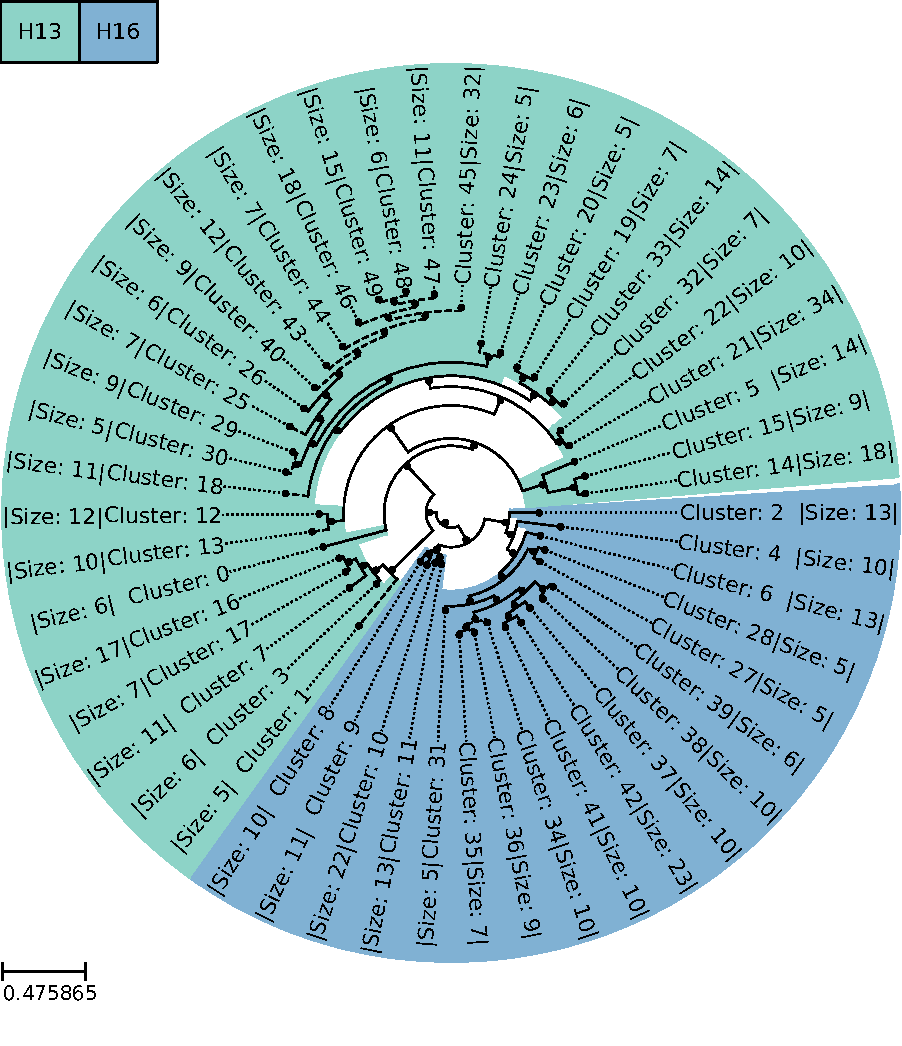
\includegraphics[width=\textwidth]{PCA/Clustertree_Segment_4_H_Cosine.pdf}
    \caption[H13/H16 Simple Clustering Example with Precalculated (cosine)]{\textbf{H13/H16 Simple Clustering Example with Precalculated (cosine).} .}
    \label{fig:Simple_Clustertree_Cosine}
\end{figure}

\begin{figure}[!hbt]
    \centering
    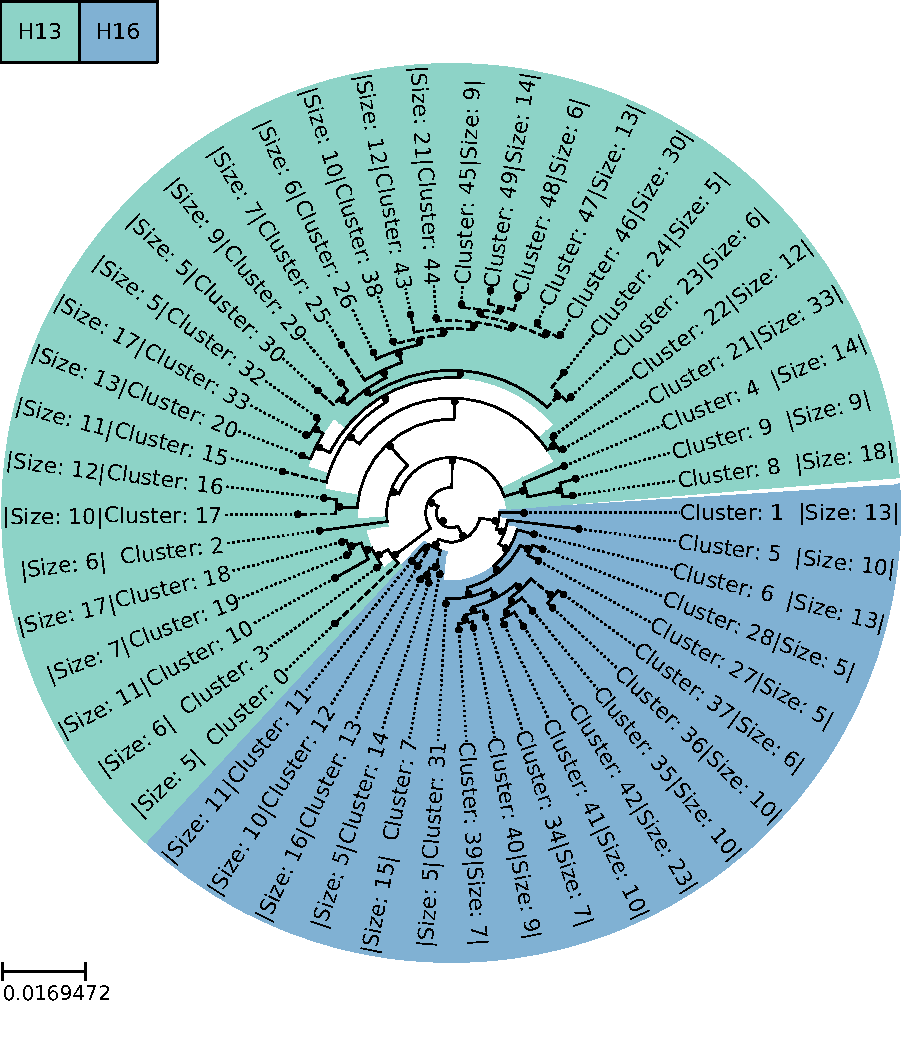
\includegraphics[width=\textwidth]{PCA/Clustertree_Segment_4_H_Euclidean.pdf}
    \caption[H13/H16 Simple Clustering Example with Precalculated (euclidean)]{\textbf{H13/H16 Simple Clustering Example with Precalculated (euclidean).} .}
    \label{fig:Simple_Clustertree_Euclid}
\end{figure}